\section{A typical session with ActarSim}
A typical ActarSim session\index{ActarSim session} contains the following procedures:
\begin{enumerate}
 \item Run ActarSim, in this step, the
 \item Run the digitizationMacro
 \item Run the analyzing macro
 \item Run the Ntuple\index{ntuple} reader to analysis the results
\end{enumerate}

\subsection{Running ActarSim}
An example of macro file needed to run ActarSim is given in section \ref{sec-ActarSim-macro}. Detailed explanations of the commands in this macro file are given in section \ref{sec-messengers}. Most of the commands and their parameters can be kept the same as in this example. The information that has to be provided by the user are the following:

\begin{enumerate}
\item The geometry\index{geometry} of chamber. Note that the numbers are \textit{half lengths} of the real geometry, for example, for a cubic chamber of $300\times300\times300$ mm$^3$, the corresponding commands are:

  \begin{verbatim}
  /ActarSim/det/gasGeoIncludedFlag on
  # if box
  /ActarSim/det/gas/setDetectorGeometry box
  /ActarSim/det/gas/setXLengthGasBox 150. mm
  /ActarSim/det/gas/setYLengthGasBox 150. mm
  /ActarSim/det/gas/setZLengthGasBox 150. mm
  \end{verbatim}

\item To include silicon and scintillator (CsI) detectors or not:
  \begin{verbatim}
  /ActarSim/det/silGeoIncludedFlag on or off
  /ActarSim/det/sciGeoIncludedFlag on or off
  \end{verbatim}
At present the geometry of ancillary detectors\index{ancillary detectors} are hard-coded, i.e., the silicon detectors are 300 $\mu$m thick and of $100\times100$ mm$^2$ square shapes, the square CsI detectors are $25\times25$ mm$^2$ and 30 mm thick. If we want to include the silicon and scintillator detectors, we also have to specify the size of ``boxes'' (usually the same length parameter as the gas chamber) to put the ancillary detectors:
  \begin{verbatim}
  /ActarSim/det/sil/sideCoverage 56
  /ActarSim/det/sil/xBoxHalfLength 150. mm
  /ActarSim/det/sil/yBoxHalfLength 150. mm
  /ActarSim/det/sil/zBoxHalfLength 150. mm

  /ActarSim/det/sci/sideCoverage 56
  /ActarSim/det/sci/xBoxHalfLength 150. mm
  /ActarSim/det/sci/yBoxHalfLength 150. mm
  /ActarSim/det/sci/zBoxHalfLength 150. mm
  \end{verbatim}
please refer to section \ref{sec-messengers} for the definition of \textit{sideCoverage}.

\item The active gas and its pressure, for example, deuterium gas at STP condition:
  \begin{verbatim}
  /ActarSim/det/gas/setGasMat D2_STP
  \end{verbatim}
The following gas/pressure\index{gas/pressure} are pre-defined in ActarSim:
  \begin{itemize}
    \item isobutane\index{isobutane}: isoC4H10STP, isoC4H10\_150, isoC4H10\_220, isoC4H10\_300, isoC4H10\_500, isoC4H10\_710, isoC4H10\_1300, and isoC4H10\_1880

    \item deuterium\index{deuterium}: D2\_40, D2\_60, D2\_80, D2\_100, to D2\_400 with steps of 20 mbar, D2\_STP, D2\_1695, D2\_1800, and D2\_1950

    \item helieum\index{helieum}:   He\_1900, and He\_2010
  \end{itemize}
where the units are in mbar.

\item What information are to be stored in the output file:
  \begin{verbatim}
   #Control of the output on the ROOT file
   #if all the tracks are stored (note: huge space comsumption)
   /ActarSim/analControl/storeTracks off
   /ActarSim/analControl/storeTrackHistos off
   /ActarSim/analControl/storeEvents on
   /ActarSim/analControl/storeHistograms off
   /ActarSim/analControl/storeSimpleTracks on
  \end{verbatim}
Usually we do not need to restore all tracks, which consumes huge hard disk space. For the ROOT macros described in the following text, only \textit{storeEvents} and \textit{storeSimpleTracks} are needed to be swifted on. With these options, the output file size is around 60 MB for a run of 5000 Geant4 events.

\item Whether we need to treat the beam energy loss\index{beam energy loss} (beam interaction) in the gas and its emittance\index{emittance} (realistic Beam):
  \begin{verbatim}
   /ActarSim/gun/beamInteraction on
   /ActarSim/gun/realisticBeam on
   /ActarSim/gun/beamRadiusAtEntrance 2.5 mm
   /ActarSim/gun/emittance 200.0
  \end{verbatim}
The unit of emittance here is mm mmrad.

\item Which reaction kinematics calculator to use. We have two options: CINE\index{CINE} and KINE. Suppose we use KINE\index{KINE}, the following commands should be issued:
  \begin{verbatim}
   /ActarSim/gun/reactionFromKine on
   /ActarSim/gun/Kine/incidentIon 28 78 28 0.0 77.96318
   /ActarSim/gun/Kine/targetIon 1 2 1 0.0 2.0141
   /ActarSim/gun/Kine/scatteredIon 28 79 28 5.0 78.97107
   /ActarSim/gun/Kine/recoilIon 1 1 1 0.0 1.007825
   /ActarSim/gun/Kine/labEnergy 624. MeV
   /ActarSim/gun/Kine/randomThetaCM on
   /ActarSim/gun/Kine/randomThetaRange 0.0 180.0
   /ActarSim/gun/Kine/randomPhiAngle on
   /ActarSim/gun/Kine/userThetaCM 41.0 deg
   /ActarSim/gun/Kine/userPhiAngle 50.0 deg
  \end{verbatim}
These commands define the entrance- and exit-channel particles to be studied. The parameters for these particles are atomic number, mass number, charge number, excitation energy (in MeV) and atomic mass (in u), respectively. The above information is for the \nuc{78}{Ni}(d,p)\nuc{79}{Ni} at incident energy of 8 AMeV with \nuc{79}{Ni} at 5 MeV of excitation. The $\theta_\text{cm}$ and $\phi$ angles are randomized (so that the values of \textit{userThetaCM} and \textit{userPhiAngle} above actually do not matter).
\end{enumerate}

There are also commands that control the visualization of the ActarSim runs, however, they are not relevant to the storage of the calculated informations. Note that enabling the visualization will greatly slow down the speed of calculation.

\subsection{The digitization macro}

The output file of ActarSim only contain information about strides of particles in the gas (data members of class \textit{ActarSimSimpleTrack}), and about the silicon and CsI detectors (data members of class \textit{ActarSimSilHit} and \textit{ActarSimSciHit}). Pad signals (charges induced and timing, data member of class \textit{ActarPadSignal}) are calculated by using a digitization\index{digitization} macro \textit{digitizationMacro.C}. This macro dose the folloing things:
\begin{enumerate}
 \item reads the output file of ActarSim event-by-event,
 \item for each event, reads the information of each stride,
 \item for each stride, calculate the corresponding pads that have induced charge on them, for each pad which has induced charge, the corresponding time for the primary electrons of this stride to drift from the ionization position to the pad plane is also calculated.
\end{enumerate}

To perform above calculations, the following information have to be passed to the digitizationMacro\index{the digitizationMacro}:

\begin{enumerate}

\item the geometry of the detector:
\begin{verbatim}
      thePadsGeometry.SetGeometryValues(Int_t geometryType,
                                        Int_t padType,
                                        Int_t padLayout,
                                        Double_t xLength,
                                        Double_t yLength,
                                        Double_t zLength,
                                        Double_t radius,
                                        Double_t padSize)
\end{verbatim}
Where all distances in this command should be included in mm. The macro calculates the number of pads in each column and row.

\item The drift velocity\index{drift velocity} and diffusion parameters\index{diffusion parameters} of electron clouds:
\begin{verbatim}
        theDriftManager.SetDriftVelocity(Double_t velocity)       in mm/ns
        theDriftManager.SetDiffusionParameters(Double_t  long,
                                               Double_t  trans)   in mm^2/ns
\end{verbatim}

\item other parameters, such as the Lorentz angle
\begin{verbatim} 
        theDriftManager.SetLorentzAngle(Double_t lor)           in radians
\end{verbatim}
\end{enumerate}

The event-loop (and inside a stride-loop) is performed for all strides\index{stride} within all events in the input root file. The projection of each stride on the pad plane is performed using the drift parameters. Then, a calculation of the (relative units) induced charge in each pad close to the projection points is performed:
\begin{verbatim}
        Int_t CalculatePositionAfterDrift(projectionOnPadPlane* pro);
        ActarPadSignal* CalculatePadsWithCharge(projectionOnPadPlane* pro,
                                           TClonesArray* clo);
\end{verbatim}

Those pads containing induced charge are stored for further analysis in a \textit{TClonesArray} stored in a TTree in an output TFile. This TFile could be used in next analysis steps (the \textit{analysisExample.C}, for example).

\subsection{Digitization in detail}

\subsubsection{Pads geometry}
The digitizationMacro calculates the number of pads using an algorithm which divides the available pad plane on the maximum number of pads with the approximate size given by the user. A small change of the pad size could be possible. The configuration and numbering of the pads are the following:

a) square pads\index{square pads}: pads are ordered in rows and columns from 1 up to the parameters \textit{numberOfRows} and \textit{numberOfColumns}. An example with 5 columns and 4 rows is shown in Fig.\ref{fig-pad-layout}-(a). In the \textit{thePadsGeometry.SetGeometryValues} function, the \textit{padType} for square pad is 0.

b) hexagonal pads\index{hexagonal pads}: pads are ordered in rows and columns from 1 up to the parameters \textit{numberOfRows} and \textit{numberOfColumns}. There are two kinds of pad layouts\index{pad layouts} for hexagonal pads: the MAYA-like (Fig.\ref{fig-pad-layout}-(b), \textit{padType==1} and \textit{padLayout==0}) and the MAYA-tilted layout (Fig.\ref{fig-pad-layout}-(c), \textit{padType==1} and \textit{padLayout==1}).

\begin{figure}[htbp]
\subfigure[square pads]{
\begin{minipage}[b]{0.32\textwidth}
\centering
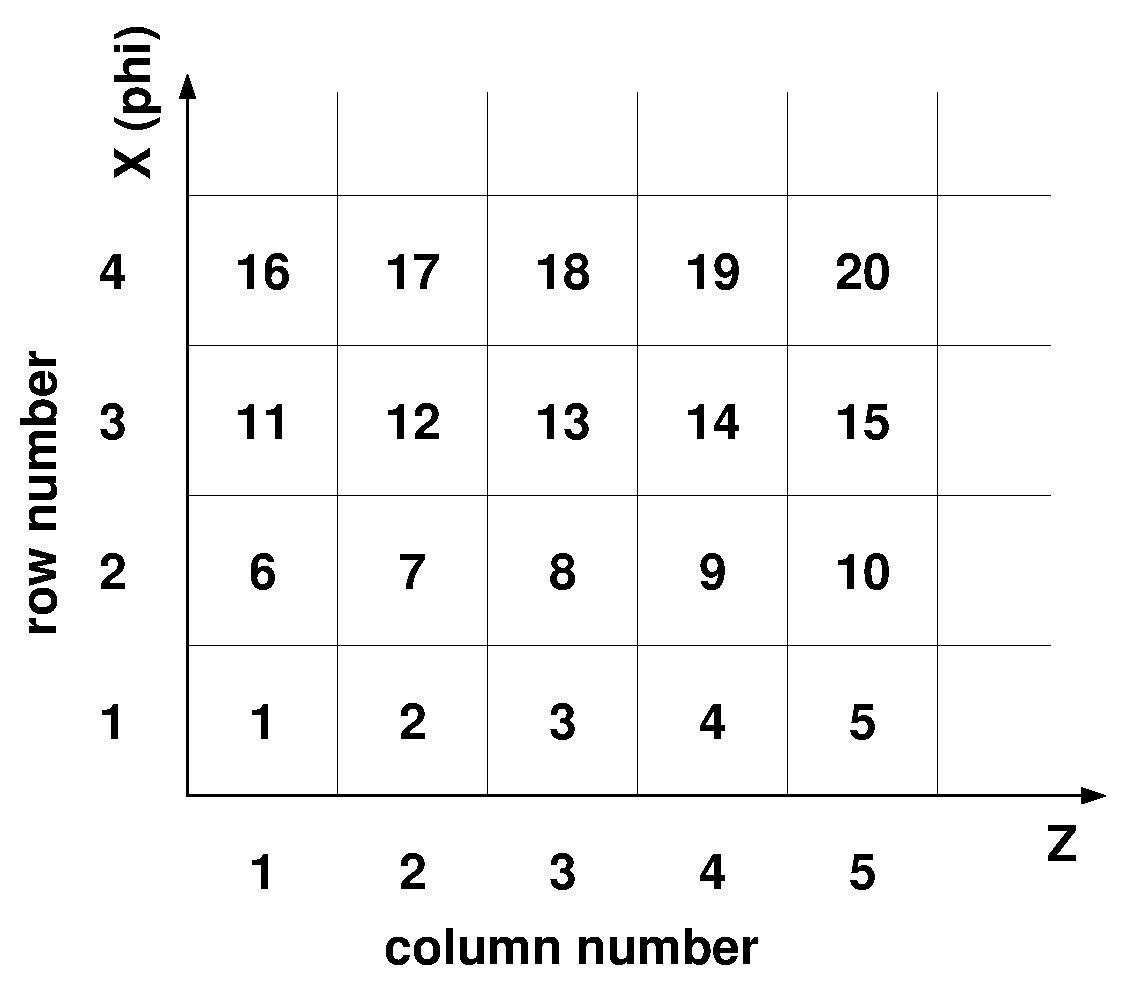
\includegraphics[width=\textwidth]{layout-squarePads.eps}
\end{minipage}}%
\subfigure[MAYA-like layout]{
\begin{minipage}[b]{0.32\textwidth}
\centering
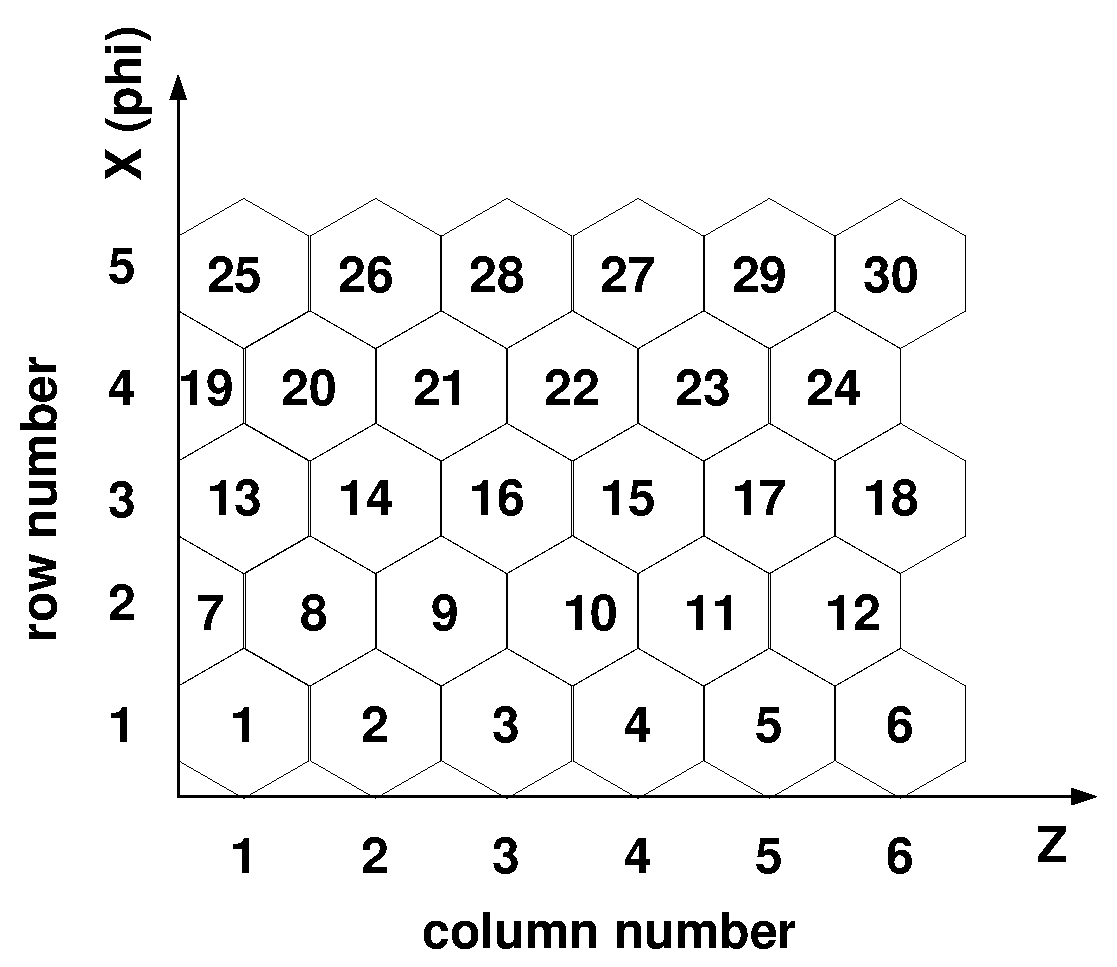
\includegraphics[width=\textwidth]{layout-mayaType.eps}
\end{minipage}}
\subfigure[MAYA-tilted layout]{
\begin{minipage}[b]{0.32\textwidth}
\centering
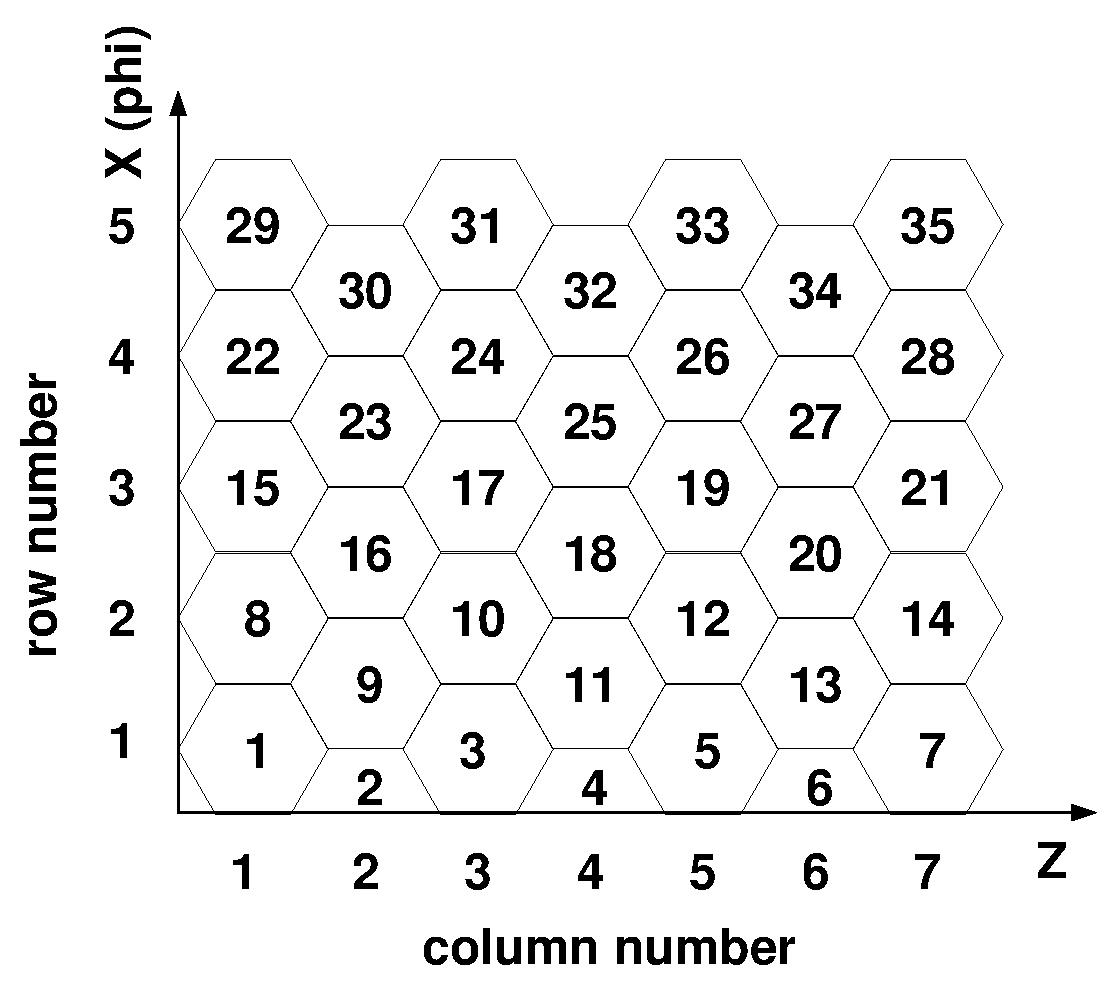
\includegraphics[width=\textwidth]{layout-hexagonal.eps}
\end{minipage}}
\caption{Pad types and layout patterns in the simulation code.}\label{fig-pad-layout}
\end{figure}

In all three cases a single number can identify the pad. The pad number is 1 for row=1, column=1, 2 for row=1, column=2, etc. A set of functions calculates the pad number from the row and column and viceversa.

\subsubsection{Drift velocity and diffusion parameters}
The electron drift velocity\index{drift velocity} and diffusion parameters\index{diffusion parameters} can be passed to the digitizationMacro by using the following commands:
\begin{verbatim}
        theDriftManager.SetDriftVelocity(Double_t velocity)       in mm/ns
        theDriftManager.SetDiffusionParameters(Double_t  long,
                                               Double_t  trans)   in mm^2/ns
\end{verbatim}

For deuterium and isobutane gases, there are analytical formula incorporated in the code to calculate these quantities. To do use these formula, instead of the two commands above, one has to use the following commands instead:
\begin{verbatim}
        theDriftManager.SetDriftParameters(Voltage,height,pressure,gasName)
\end{verbatim}
where, for MAYA-like ACTAR detector, \textit{Voltage} (in volts) is the voltage between the upper cathode and the Frish grid, \textit{height} (in mm) is the distance between the upper cathode and the Frish grid, \textit{pressure} (in mbar) is the pressure of the active gas, and \textit{gasName} is the name of the active gas, it has only two optional values: ``deuterium'' and ``isobutane''. At the end of function \textit{theDriftManager.SetDriftParameters()} the drift velocity and diffusion parameters will be automatically calculated.

The analytical formula for deuterium and isobutane gases were obtained by fitting the corresponding curves in ref.\cite{Peisert-Sauli}. More detailed description of these formula can be found in the \textit{ActarSim-report} by D.Y. Pang.

\subsubsection{Digitization stride-by-stride}
In digitizationMacro, a loop on all events is made for the Tree in the input TFile. Inside each event, a loop on all \textit{ActarSimSimpleTracks} (strides) is performed. For each stride, an object of the class \textit{projectionOnPadPlane} is assigned. This class contains a pointer to the stride, vectors containing the projection on the pad plane for the initial and final points of the stride and the corresponding drift times for each point. Also the values of the longitudinal and transversal sigma of the diffusion distributions is contained.

All this projections and quantities are obtained from the original stride and the geometrical and drift parameters. Actually is the \textit{driftManager} class which calculates them from the original stride using the function:
\begin{verbatim} 
        theDriftManager.CalculatePositionAfterDrift(projection)
\end{verbatim}

Next, the charge induced by the electron drift on the pads is calculated. For this, a candidate pad list is prepared incuding those between the initial and final pads where the projections of the stride lie. A few neighbouring pads are included in the list (by introducing the \textit{securityFactor}) to account for the possible pads diagonal to the initial or final points. Presently, the charge is obtained from the integral of a two dimensional function, which describes the distribution of the induced charges on the pad plane, on the area of the pad (for hexagonal pads, we are using an approximating square limits in the integration -- since it is much more complicated to describe the limits of a hexagonal pad). The form of this function depends on the induction mode (wire, MicroMegas, GEM).
To perform this calculation, the function:
\begin{verbatim}
        theDriftManager.CalculatePadsWithCharge(projection,padSignalCA)
\end{verbatim}
should be called on the event loop.

\subsubsection{The wire induction mode}
In case of wire amplification\index{wire induction mode}, the induced charge distributions, parallel and normal to the wire direction, as a function of the distance between the center of the amplification $x$, are $\rho_1(x)$ and $\rho_2(x)$, respectively. According to the empirical formula of E. Mathieson and J.S. Gordon \cite{Mathieson-NIM-1984, Mathieson-NIMA-1988}, $\rho_1(x)$ and $\rho_2(x)$ are:
\begin{eqnarray}\label{eq-wire-induction}
 \rho(\lambda) &=& q_a\times{}K_1\frac{1-\tanh^2(K_2\lambda)}{1+K_3\tanh^2(K_2\lambda)},\nonumber\\
 K_1 &=& \frac{K_2\sqrt{K_3}}{4\tan^{-1}\sqrt{K_3}},\quad\textrm{and}\\
 K_2 &=& \frac{\pi}{2}\left(1-\frac{\sqrt{K_3}}{2}\right)\nonumber,
\end{eqnarray}
where $q_a$ is the net anode charge, $\lambda=x/h$ with $h$ being the distance between the anode wire plane and the cathode pad plane. To calculate the distributions of induced charge on pads using Eq.(\ref{eq-wire-induction}), the only thing needed is the value of Mathieson factor $K_3$.

The Mathieson factor\index{Mathieson factor} $K_3$ is a function of $r_a/s$ and $h/s$, where $r_a$ and $s$ are radius of the amplification wire and the distance between two neighbouring wires, respectively. Details of calculations of $K_3$ can be found in the \textit{ActarSim-report} by D.Y. Pang. If one want to use wire induction mode, in running of the digitizationMacro, one need to issue the following two commands:
\begin{verbatim}
    theAmplificationManager.SetIsWireOn()
    theAmplificationManager.SetWireAmplificationParameters(0.02,2.,3.)
\end{verbatim}
where the first command switch the wire induction mode on, and the second command passes the wire parameters, $r_a$, $s$ and $h$ to the program (units in mm). In the above example, $r_a=20$ $mu$m, $s=2$ mm and $h=3$ mm, respectively.

\subsubsection{A complete example of running the digitizationMacro}
As explained above, below is one complete example to run the digitizationMacro\index{the digitizationMacro}:
\begin{verbatim}
    $ root -l
    root [0] gSystem->Load("actarsim.sl");
    root [1] .L digitizationMacro.C++
    root [2] thePadsGeometry.SetGeometryValues(0,0,0,150.,150.,150.,100.,2)
    root [3] theDriftManager.SetDriftParameters(10000.,300.,1013.25,"deuterium")
    root [4] theAmplificationManager.SetIsWireOn()
    root [5] theAmplificationManager.SetWireAmplificationParameters(0.02,2.,3.)
    root [6] digitEvents("simData.root","digiData.root",0)
\end{verbatim}
By doing this, we use the digitizationMacro to read the ActarSim output file \textit{simData.root} and write the resulting digitization file into \textit{digiData.root}. The active target ges is deuterium at 1 atm pressure. We are using wire induction mode with wire radius of 0.02 mm, intervals between wires are 2 mm and the wire plane is 3 mm above the pad plane.

\subsection{An example of analyzing macro}
After the digitization, we have the \textit{simulation data} which is equivalent to the experimental data. The simulation data is stored in two file: ancillary detector\index{ancillary detector} signals (silicon and CsI) are stored in the output file of ActarSim (\textit{simData.root}) and pad signals\index{pad signals} (induced charge and time) are stored in the output file of the digitizationMacro (\textit{digiData.root}). Both files are written in a event-by-event way and events related to the same reaction have the same event ID in both files.

In principle, all algorithms developed in the analysis of the MAYA experiment should be able to be applied to the simulation data in the simData.root and digiData.root files. We provide an example macro \textit{analysisExample.C} for this purpose.

For \nuc{78}{Ni} induced $(d,p)$, $(d,d^\prime)$ and $(d,t)$ reactions, the analysisExample macro reconstruct the trajectory\index{trajectory} of the light particle, i.e., proton, deuteron, and triton. From each reaction that the trajectory of the light particle is reconstructable, the analysisExample macro reads the energy signal in silicon and CsI detectors and calculates the range \index{range} of that particle inside the gas. Once the trajectory is known, the $\theta_\text{Lab}$ and $\phi$ angle of the out-going particle in the laboratory system are able to calculated and be compared with their corresponding ``real'' values and then we are able to analysis the angular resolution\index{angular resolution} of the detector for a given gas/pressure, pad information (pad size, shape and pattern of layout), and induction mode. Similarly, the position resolution\index{position resolution} can also be obtained by comparing the reconstructed reaction vertex $Z$-value with its ``real'' value given by Geant4.

To run this macro, the following ROOT command should be used:
\begin{verbatim}
    $ root -l
    root [0] gSystem->Load("actarsim.sl");
    root [1] .L analysisExample.C++
    root [2] thePadsGeometry.SetGeometryValues(0,0,0,150.,150.,150.,100.,2)
    root [3] theDriftManager.SetDriftParameters(10000.,300.,1013.25,"deuterium")
    root [4] reader("simData.root","digiData.root","Ntuples.root",1000.,3,2,0,0,0)
\end{verbatim}

Note that the arguments for functions \textit{SetGeometryValues()} and \textit{SetDriftParameters()} should be the same as the ones used in the corresponding digitizationMacro. The arguments for the function \textit{reader()} are
\begin{enumerate}
 \item simData.root: the output file of ActarSim
 \item digiData.root: the output file of the digitizationMacro
 \item Ntuples.root: the output of this analysisExample macro, in which the following information are stored reaction-by-reaction in a TNtuple\index{ntuple}:
 \begin{itemize}
  \item G4VertexZ: the $Z$-value of the reaction vertex given by Geant4
  \item G4ThetaLab: the $\theta_\text{Lab}$ of the out-going light particle given by Geant4
  \item G4PhiLab: the $\phi$ angle of the out-going light particle given by Geant4
  \item G4VertexE: the beam energy at the reaction vertex given by Geant4 (taking into account the beam energy loss in the gas)
  \item calVertexZ: the $Z$-value of the reaction vertex from the reconstructed particle trajectory
  \item calThetaLab: the $\theta_\text{Lab}$ of the out-going light particle from the reconstructed particle trajectory
  \item calPhiLab: the $\phi$ angle of the out-going light particle from the reconstructed particle trajectory
  \item eSil: the energy loss of the light particle inside the silicon detector (in MeV)
  \item eSci: the energy loss of the light particle inside the CsI detector (in MeV)
  \item protonRangeInGas: the proton range inside the gas (in mm), note that the range is calculated whenever the trajectory of the particle is reconstructable, it does not mean that the particle is stopped inside the gas.
 \end{itemize}

 \item the dynamic range\index{dynamic range}: ratio between the maximum and minimum charge signals that can be measured on the pads. In this analysisExample macro, we determine the minimum charge on the pads by dividing the maximum charge with the dynamic range. This is equivalent to the thresholds\index{thresholds}. In the above example, dynamic range is 1000.

 \item the beam projection width\index{beam projection width} (bw): half of the number of rows of pads that are taken by the beam, the trajectory of light particles is not be able to be reconstructed if its projection on pad plane falles between $[\text{numberOfRows}/2-\text{bw}, \text{numberOfRows}/2+\text{bw}]$. In the above example, bw is 3.

\item the margin width\index{margin width} (mw): number of rows and columns at the edges of the gas chamber. We do not take the signals of the ``margin pads'' as effective singals. In the above example, mw is 2.

\item the last three zeroes in the arguments of the function reader() are verbose level, minimun and maximum reaction numbers (minReactionNumber and maxReactionNumber), respectively. If the verbose level is larger or equal to 1, the program will give some diagnosis information, which is useful if we want to know the details of the running of this macro. If minReactionNumber and maxReactionNumber are zeroes, all reactions will be treated, otherwise, only reactions with reaction number between the minReactionNumber and maxReactionNumber will be treated. In the above example, we include all reactions in the analysis.
\end{enumerate}

In this analysisExample macro, seven histograms\index{histogram} are defined, namely:
\begin{itemize}
\item hLightEvsTheta: two dimensional, $E-\theta_\text{Lab}$ kinematics plot for the out-going light particle, where $E$ are energy signals in ancillary detectors.

\item hDThetavsTheta: two dimensional, $\Delta\theta_\text{Lab}-\theta_\text{Lab}$, this histogram shows how the difference between ``real'' value of $\theta_\text{Lab}$ and its reconstructed value ($\Delta\theta_\text{Lab}$) depends on the value $\theta_\text{Lab}$ itself.

\item hDThetavsPhi: two dimensional, $\Delta\theta_\text{Lab}-\phi$, this histogram shows how $\Delta\theta_\text{Lab}$ depends on the reconstructed $\phi$ value.

\item hRangeVSTheta: two dimensional, correlation between the range of the light particle and its $\theta_\text{Lab}$.

\item hDTheta: one dimensional, angular resolution\index{angular resolution} in $\theta_\text{Lab}$

\item hDPhi: one dimensional, angular resolution in $\phi$

\item hDVertexZ: one dimensional, position resolution\index{position resolution} in reaction vertex $Z$-value.
\end{itemize}

The users of ActarSim can define their own histograms. It is more useful to study the correlations between quantities we are interested in. This can be done by using TNtuples.

\subsection{An example of TNtuple reader}

The analysisExample macro generate an output ROOT file which contains one TNtuple. The contents of this ntuple\index{ntuple} has been introduced in the previous section. We provide the macro \textit{ntupleReader.C} as an example of manipulate these ntuple data members. In this macro we can include as many number of runs of simulation and analysis them together. For example, the $(d,p)$, $(d,d^\prime)$ and $(d,t)$ reactions are simulated in different runs, we can use this macro to put analysis these reactions together.

Some example of the analyzing result using the analysisExample and ntupleReader macros can be find in the \textit{\nuc{78}{Ni}-dp-simulation-report} file by D.Y. Pang.
